\section[Motivation]{Motivation}

% \begin{frame}
%   \frametitle{Polymer solutions}
%   \begin{columns}
%     \begin{column}{0.5\textwidth}
%       \begin{block}{Polymer solutions}
%         \begin{itemize}
%         \item Turbulent drag reduction
%         \item Elastic instabilities and elastic turbulence leads to efficient mixing in microchannel flow
%         \end{itemize}
%       \end{block}
%       \begin{block}{Why SPH?}
%         \begin{itemize} 
%         \item Direct presentation of conformation of polymer molecules
%         \item Easy measurement of elastic stress field
%         \end{itemize}
%       \end{block}
%     \end{column}
%     \begin{column}{0.5\textwidth}
%       \begin{figure}[t]
%         \centering
%         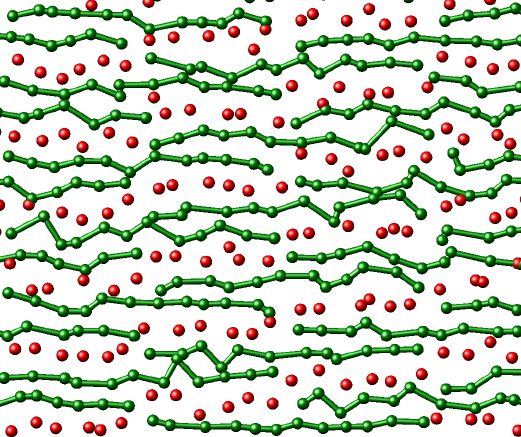
\includegraphics[width=0.6\textwidth]{img/polymers.png}
%         \caption{Snapshot of polymer solutions in 2D}
%         \label{fig:snap}
%       \end{figure}
%     \end{column}
%   \end{columns}
% \end{frame}

\begin{frame}
  \frametitle{Instabilities in polymer solutions}
  \begin{columns}
    \begin{column}{0.5\textwidth}
      \begin{figure}[t]
        \centering
        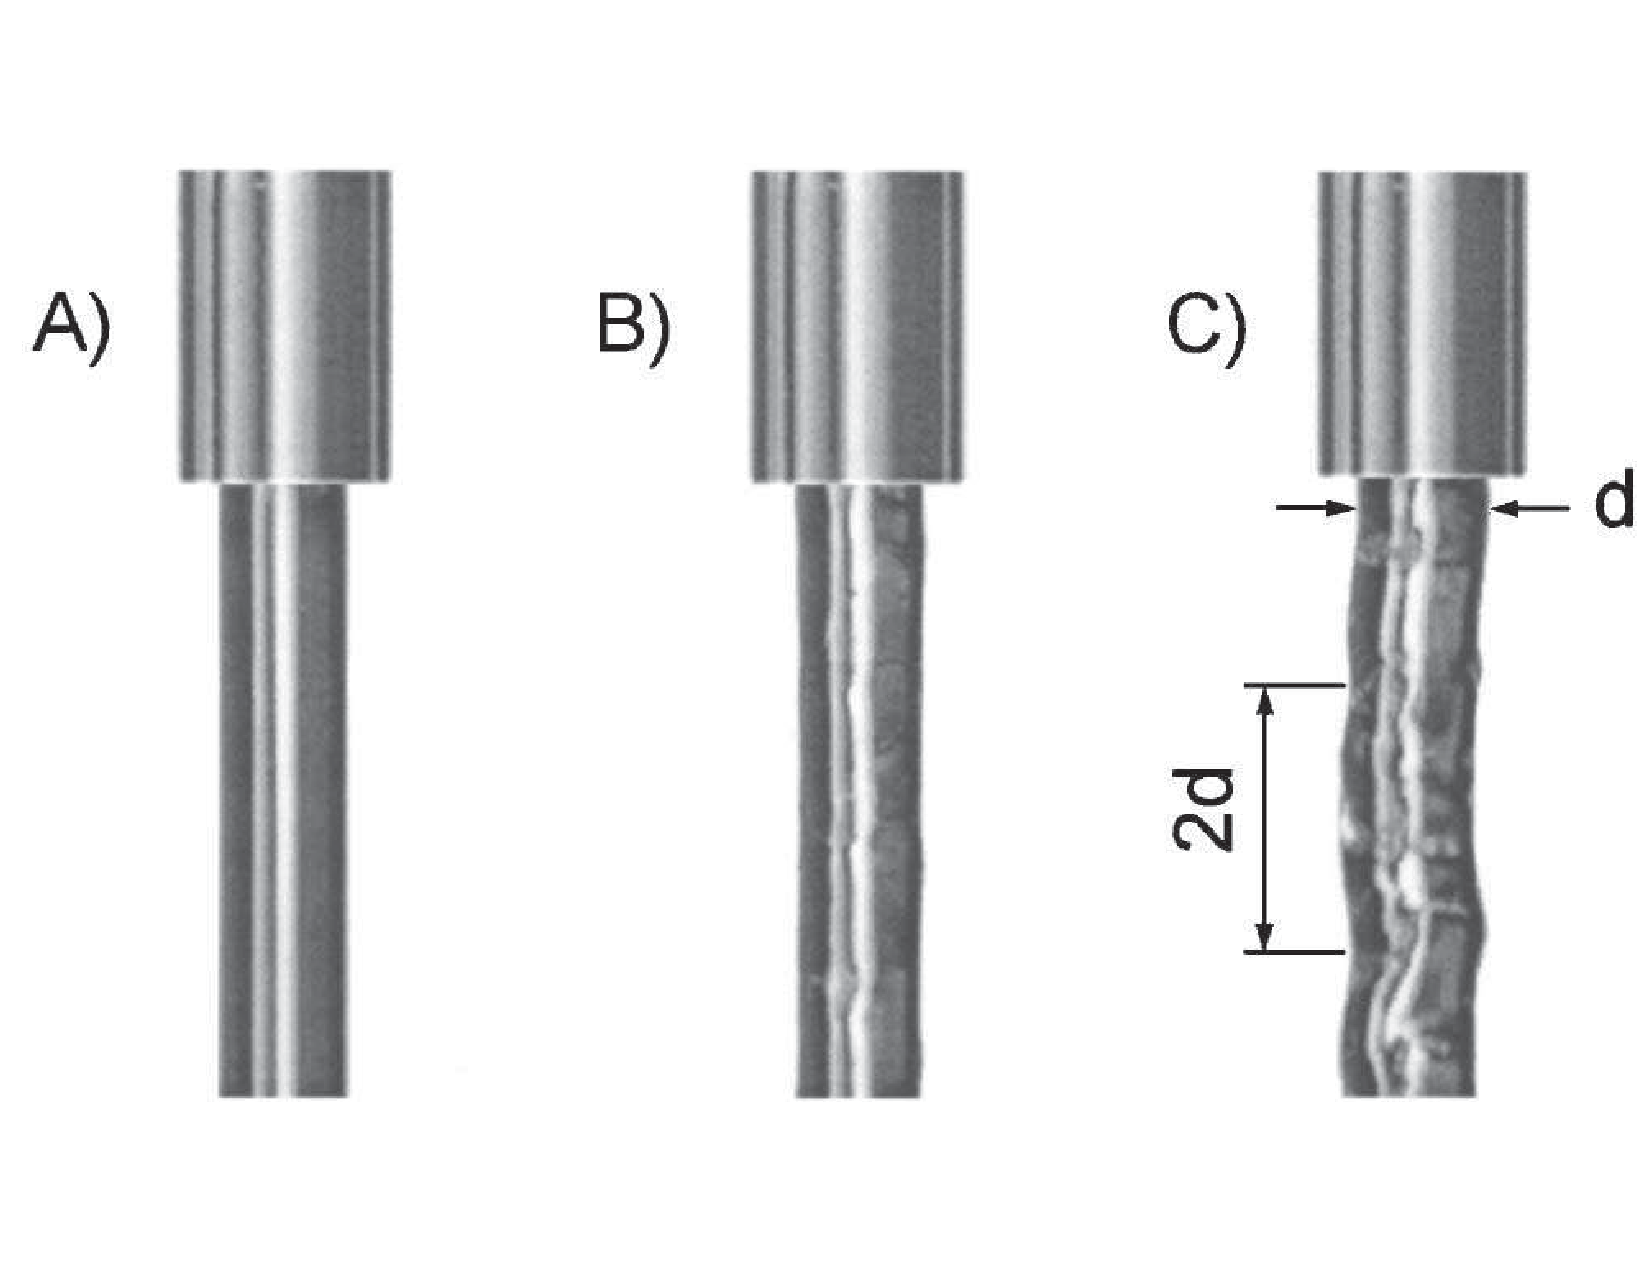
\includegraphics[width=0.8\textwidth]{img/melt.pdf}
        \caption{\alert{Bad}: The extrusion for different speed ($Wi=2.8, 4.9,
          8.4$)~\footnotemark}
        \label{fig:snap}
      \end{figure}
    \end{column}
    \begin{column}{0.5\textwidth}
      \begin{figure}[t]
        \centering
        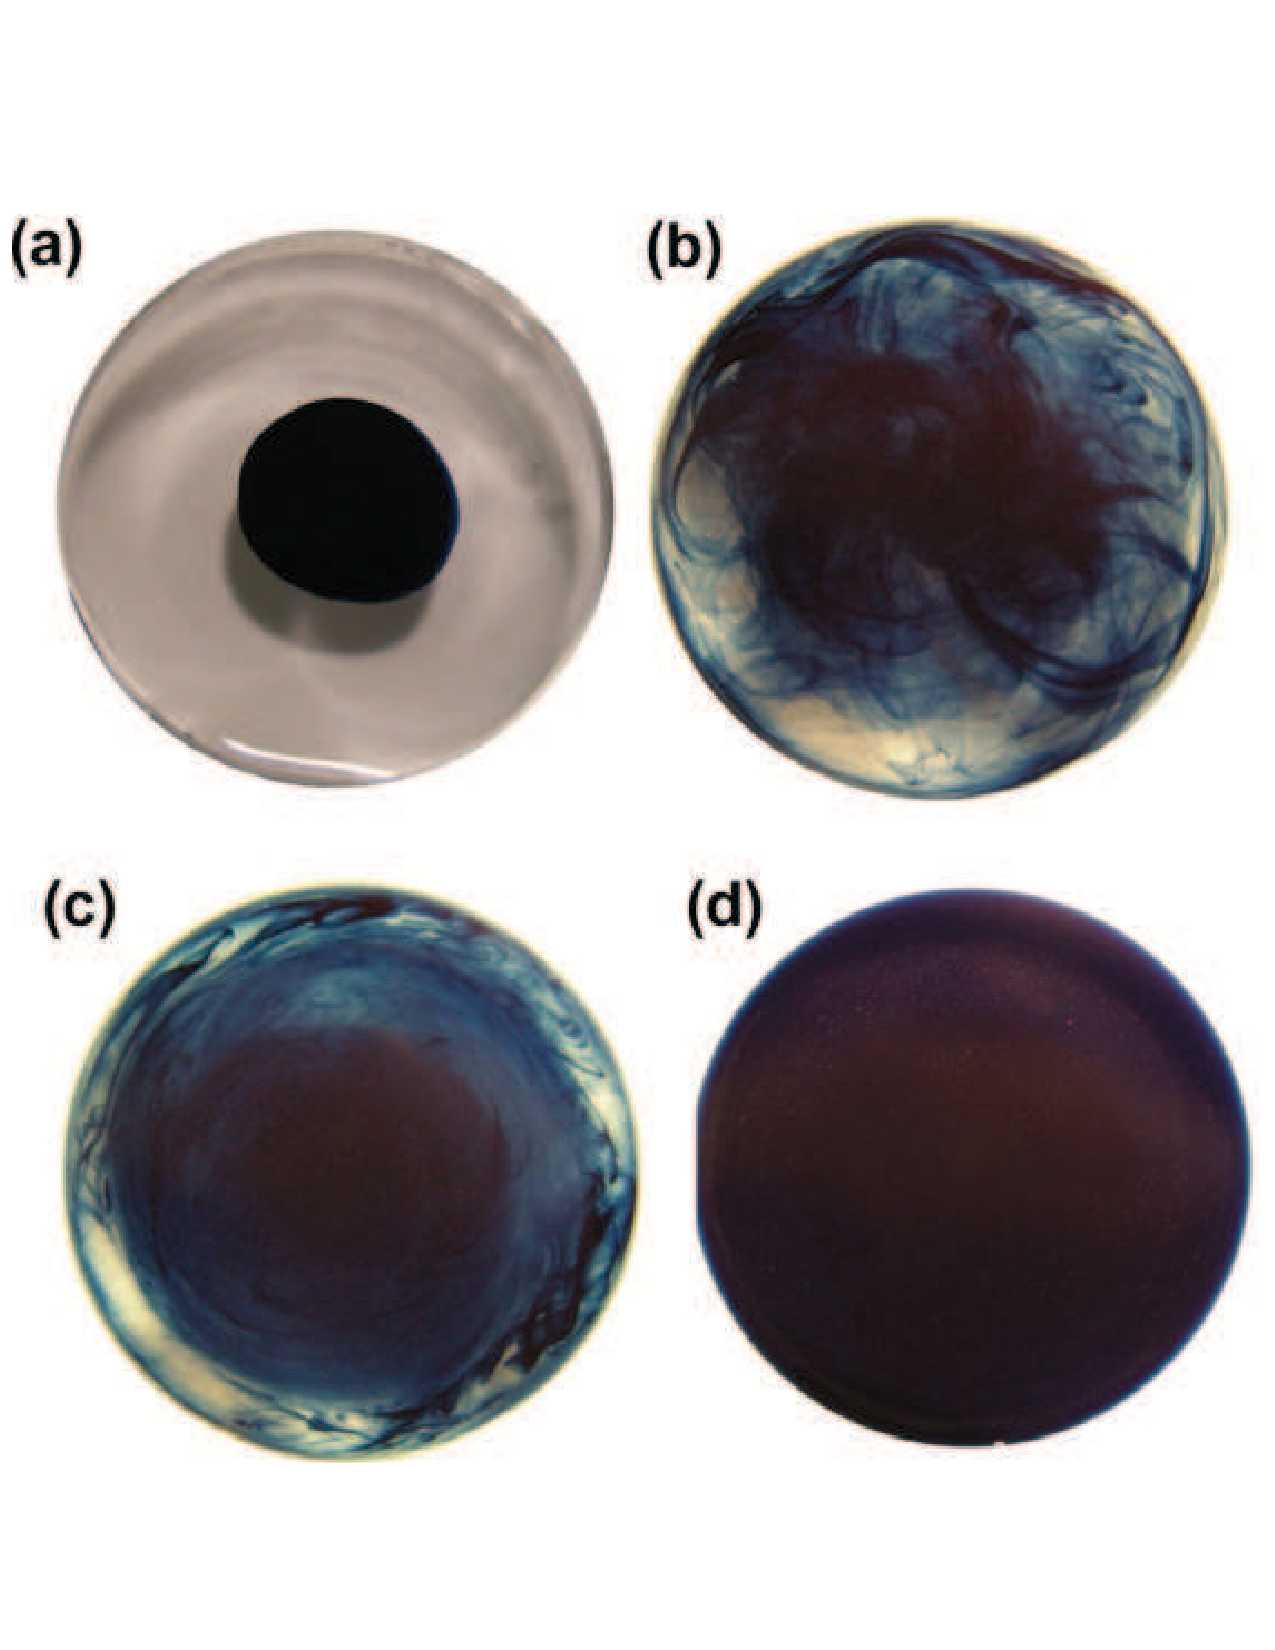
\includegraphics[width=0.7\textwidth]{img/mix2.pdf}
        \caption{\alert{Good}: Mixing of passive scalar in polymer solution~\footnotemark}
        \label{fig:snap}
      \end{figure}
    \end{column}
  \end{columns}
\footnotetext[1]{\tiny \bibentry{bertola2003experimental}}
\footnotetext[2]{\tiny \bibentry{poole2012emulsification}}
\end{frame}

\begin{frame}
  \frametitle{Motivation}
  \begin{block}{Properties of elastic instabilities}
    \begin{itemize}
    \item not inertia-driven
    \item chaotic and similar to inertia-turbulence (Elastic Turbulence)
    \item caused by interactions between polymer molecules and flow
    \end{itemize}
  \end{block}
  \begin{block}{Why study? (A. Morozov, U. Edinburgh)}
    \begin{itemize}
    \item possibly, a new type of turbulence
    \item applications
    \item we can learn about inertia-turbulence
    \end{itemize}
  \end{block}
\end{frame}

% \begin{frame}
%   \frametitle{Motivation}
%   \begin{block}{Why (Four)-Roll Mill Flow?}
%     \begin{itemize}
%     \item Extensional flow is more effective to locally 
%       stretch polymer molecules than simple shear flow
%     \item Polymer molecules are strongly stretched at extensional points in a micro-channel cross flow
%     \end{itemize}
%   \end{block}
%   The four-roll mill flow is driven by a steady background force in 2D:
%   \begin{equation}
%     \mathbf{F}=\left\{\begin{matrix}
%         C_0\sin(\frac{2\pi x} {L})\cos(\frac{2\pi x} {L})
%         \\ 
%         -C_0\cos(\frac{2\pi x} {L})\sin(\frac{2\pi x} {L})
%       \end{matrix}\right.
%   \end{equation}
% \end{frame}

\begin{frame}
  \frametitle{Four-roller mill}
  \begin{columns}
    \begin{column}{0.3\textwidth}
      \begin{figure}[t]
        \centering
        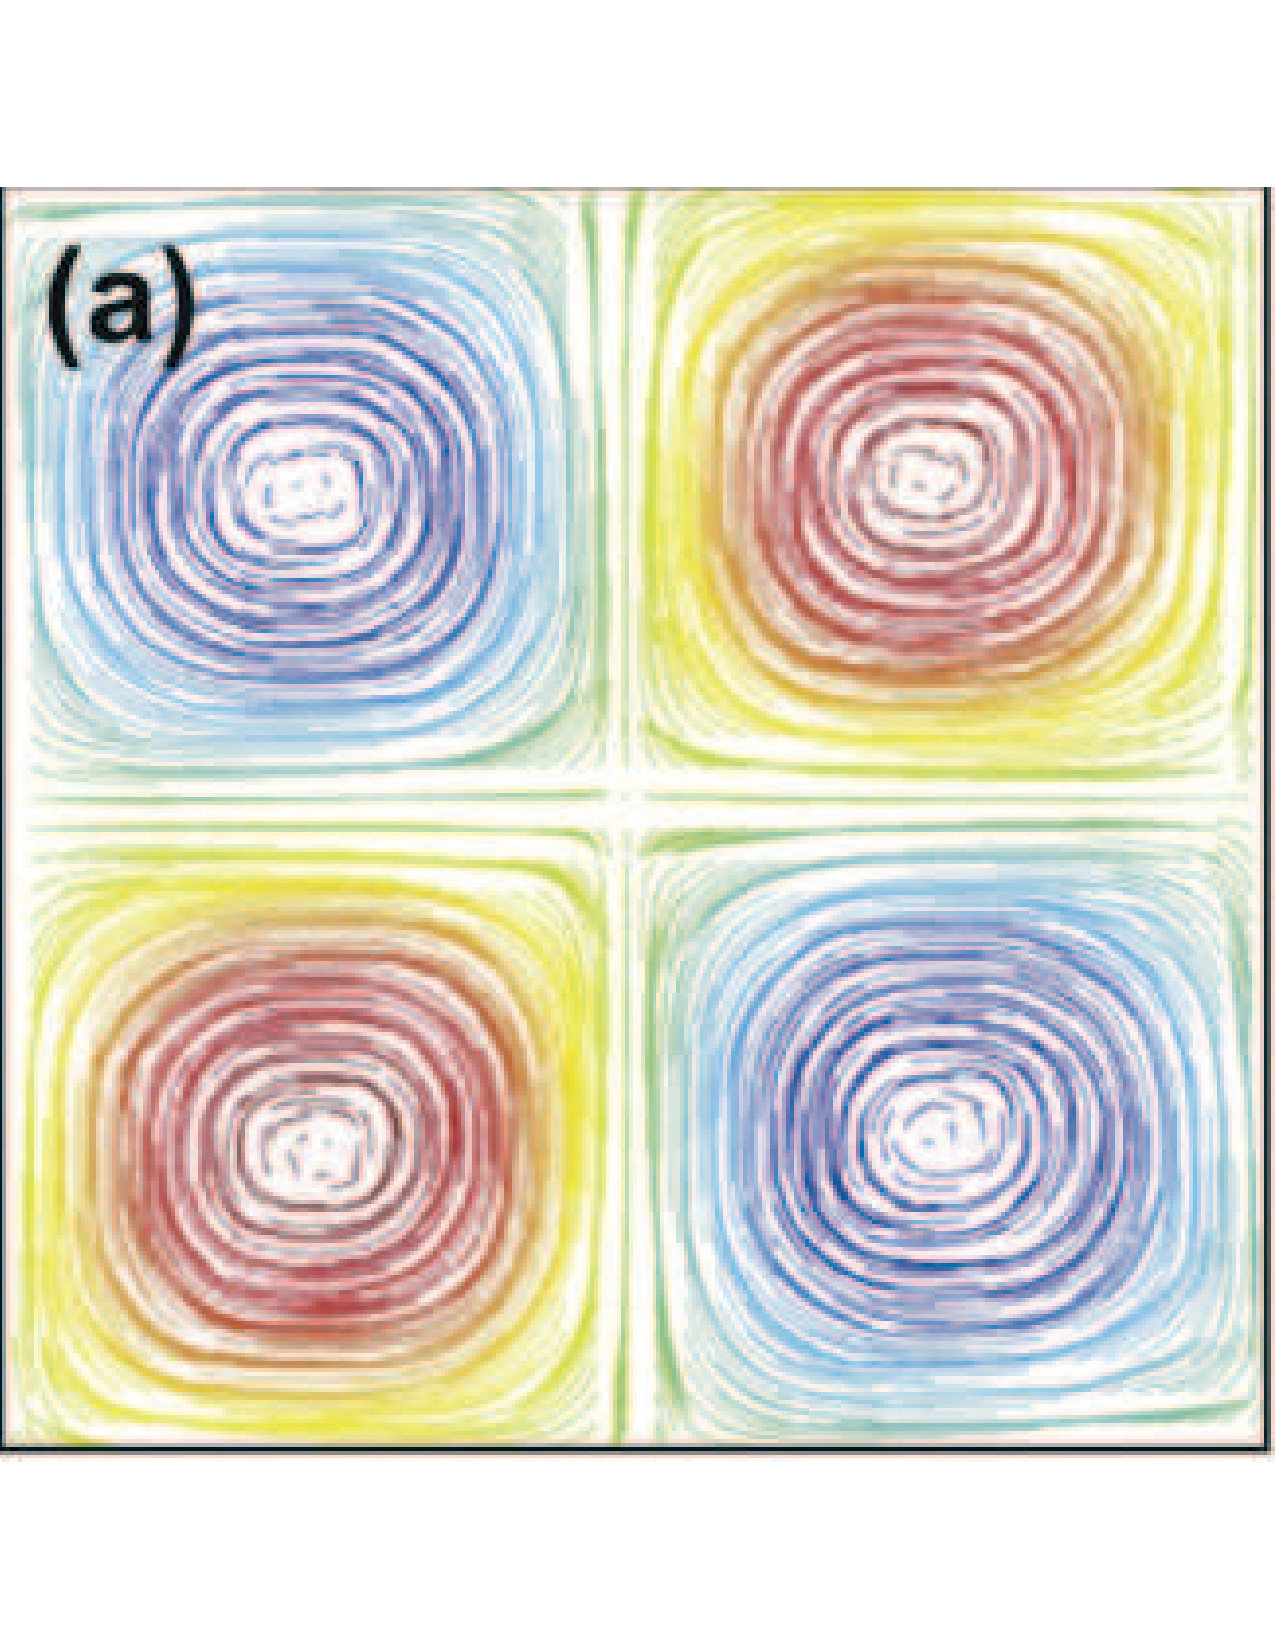
\includegraphics[width=0.9\textwidth]{img/4roll.pdf}
        \caption{``Four-roller mill'' flow field}
        \label{fig:snap}
      \end{figure}
    \end{column}
    \begin{column}{0.7\textwidth}
      \begin{block}{Why Four-Roll Mill Flow?}
        \begin{itemize}
        \item Experimental data
        \item Extensional flow is effective to  stretch polymers
        \item Easy to simulate: periodic boundaries + time-constant external force
          \begin{equation*}
            \mathbf{F}=\left\{\begin{matrix}
                C_0\sin(\frac{2\pi x} {L})\cos(\frac{2\pi y} {L})
                \\ 
                -C_0\cos(\frac{2\pi x} {L})\sin(\frac{2\pi y} {L})
              \end{matrix}\right.
   \end{equation*}
     \end{itemize}
      \end{block}
    \end{column}
  \end{columns}
\end{frame}

\begin{frame}
  \frametitle{Related Work}
  \begin{block}{Experiments by Liu et al.~\footnotemark[2]:}
    \begin{itemize}
    \item  At low Wi the flow pattern is nearly Newtonian. 
    \item At higher Wi, the strength and the position of the vortices fluctuates periodically.
    \item At even higher Wi, the flow field fluctuates stochastically in space and time.
    \end{itemize}
  \end{block}
  \begin{block}{Numerical Simulation by Thomases et al. with DNS~\footnotemark: }
    \begin{itemize}
    \item Beyond a first critical Wi number, the flow near the stagnation point becomes asymmetric and stretched.
    \item At higher Wi number, the flow is dominated by a single large vortex and persistent oscillations occur. 
    \end{itemize}
  \end{block}
  \footnotetext{\tiny \bibentry{Thomases2011}}
  \footnotetext[2]{\tiny \bibentry{Liu2012}}
\end{frame}


% \begin{frame}
%   \frametitle{Models}
%   \begin{itemize}
%   \item VOF \\
%     \bibintext{welch_local_1995}, \\
%     \bibintext{kunkelmann_cfd_2009}
%   \item Lattice Boltzmann \\
%     \bibintext{markus_pool_2012}
%   \item Particle-Based \\
%     \bibintext{muller_particle-based_2005}, \\ 
%    \bibintext{yoon_direct_2001}
%   \end{itemize}
% \end{frame}

%%% Local Variables: 
%%% mode: latex
%%% TeX-master: t
%%% End: 
